% Template for PLoS
% Version 3.5 March 2018
%
% % % % % % % % % % % % % % % % % % % % % %
%
% -- IMPORTANT NOTE
%
% This template contains comments intended 
% to minimize problems and delays during our production 
% process. Please follow the template instructions
% whenever possible.
%
% % % % % % % % % % % % % % % % % % % % % % % 
%
% Once your paper is accepted for publication, 
% PLEASE REMOVE ALL TRACKED CHANGES in this file 
% and leave only the final text of your manuscript. 
% PLOS recommends the use of latexdiff to track changes during review, as this will help to maintain a clean tex file.
% Visit https://www.ctan.org/pkg/latexdiff?lang=en for info or contact us at latex@plos.org.
%
%
% There are no restrictions on package use within the LaTeX files except that 
% no packages listed in the template may be deleted.
%
% Please do not include colors or graphics in the text.
%
% The manuscript LaTeX source should be contained within a single file (do not use \input, \externaldocument, or similar commands).
%
% % % % % % % % % % % % % % % % % % % % % % %
%
% -- FIGURES AND TABLES
%
% Please include tables/figure captions directly after the paragraph where they are first cited in the text.
%
% DO NOT INCLUDE GRAPHICS IN YOUR MANUSCRIPT
% - Figures should be uploaded separately from your manuscript file. 
% - Figures generated using LaTeX should be extracted and removed from the PDF before submission. 
% - Figures containing multiple panels/subfigures must be combined into one image file before submission.
% For figure citations, please use "Fig" instead of "Figure".
% See http://journals.plos.org/plosone/s/figures for PLOS figure guidelines.
%
% Tables should be cell-based and may not contain:
% - spacing/line breaks within cells to alter layout or alignment
% - do not nest tabular environments (no tabular environments within tabular environments)
% - no graphics or colored text (cell background color/shading OK)
% See http://journals.plos.org/plosone/s/tables for table guidelines.
%
% For tables that exceed the width of the text column, use the adjustwidth environment as illustrated in the example table in text below.
%
% % % % % % % % % % % % % % % % % % % % % % % %
%
% -- EQUATIONS, MATH SYMBOLS, SUBSCRIPTS, AND SUPERSCRIPTS
%
% IMPORTANT
% Below are a few tips to help format your equations and other special characters according to our specifications. For more tips to help reduce the possibility of formatting errors during conversion, please see our LaTeX guidelines at http://journals.plos.org/plosone/s/latex
%
% For inline equations, please be sure to include all portions of an equation in the math environment.  For example, x$^2$ is incorrect; this should be formatted as $x^2$ (or $\mathrm{x}^2$ if the romanized font is desired).
%
% Do not include text that is not math in the math environment. For example, CO2 should be written as CO\textsubscript{2} instead of CO$_2$.
%
% Please add line breaks to long display equations when possible in order to fit size of the column. 
%
% For inline equations, please do not include punctuation (commas, etc) within the math environment unless this is part of the equation.
%
% When adding superscript or subscripts outside of brackets/braces, please group using {}.  For example, change "[U(D,E,\gamma)]^2" to "{[U(D,E,\gamma)]}^2". 
%
% Do not use \cal for caligraphic font.  Instead, use \mathcal{}
%
% % % % % % % % % % % % % % % % % % % % % % % % 
%
% Please contact latex@plos.org with any questions.
%
% % % % % % % % % % % % % % % % % % % % % % % %

\documentclass[10pt,letterpaper]{article}
\usepackage[top=0.85in,left=2.75in,footskip=0.75in]{geometry}

% amsmath and amssymb packages, useful for mathematical formulas and symbols
\usepackage{amsmath,amssymb}

% Use adjustwidth environment to exceed column width (see example table in text)
\usepackage{changepage}

% Use Unicode characters when possible
\usepackage[utf8x]{inputenc}

% textcomp package and marvosym package for additional characters
\usepackage{textcomp,marvosym}

% cite package, to clean up citations in the main text. Do not remove.
\usepackage{cite}

% Use nameref to cite supporting information files (see Supporting Information section for more info)
\usepackage{nameref,hyperref}

% line numbers
\usepackage[right]{lineno}

% ligatures disabled
\usepackage{microtype}
\DisableLigatures[f]{encoding = *, family = * }

% color can be used to apply background shading to table cells only
\usepackage[table]{xcolor}

% array package and thick rules for tables
\usepackage{array}

% create "+" rule type for thick vertical lines
\newcolumntype{+}{!{\vrule width 2pt}}

% create \thickcline for thick horizontal lines of variable length
\newlength\savedwidth
\newcommand\thickcline[1]{%
	\noalign{\global\savedwidth\arrayrulewidth\global\arrayrulewidth 2pt}%
	\cline{#1}%
	\noalign{\vskip\arrayrulewidth}%
	\noalign{\global\arrayrulewidth\savedwidth}%
}

% \thickhline command for thick horizontal lines that span the table
\newcommand\thickhline{\noalign{\global\savedwidth\arrayrulewidth\global\arrayrulewidth 2pt}%
	\hline
	\noalign{\global\arrayrulewidth\savedwidth}}


% Remove comment for double spacing
%\usepackage{setspace} 
%\doublespacing

% Text layout
\raggedright
\setlength{\parindent}{0.5cm}
\textwidth 5.25in 
\textheight 8.75in

% Bold the 'Figure #' in the caption and separate it from the title/caption with a period
% Captions will be left justified
\usepackage[aboveskip=1pt,labelfont=bf,labelsep=period,justification=raggedright,singlelinecheck=off]{caption}
\renewcommand{\figurename}{Fig}

% Use the PLoS provided BiBTeX style
\bibliographystyle{plos2015}

% Remove brackets from numbering in List of References
\makeatletter
\renewcommand{\@biblabel}[1]{\quad#1.}
\makeatother



% Header and Footer with logo
\usepackage{lastpage,fancyhdr,graphicx}
\usepackage{epstopdf}
%\pagestyle{myheadings}
\pagestyle{fancy}
\fancyhf{}
%\setlength{\headheight}{27.023pt}
%\lhead{\includegraphics[width=2.0in]{PLOS-submission.eps}}
\rfoot{\thepage/\pageref{LastPage}}
\renewcommand{\headrulewidth}{0pt}
\renewcommand{\footrule}{\hrule height 2pt \vspace{2mm}}
\fancyheadoffset[L]{2.25in}
\fancyfootoffset[L]{2.25in}
\lfoot{\today}

%% Include all macros below

\newcommand{\lorem}{{\bf LOREM}}
\newcommand{\ipsum}{{\bf IPSUM}}

%% END MACROS SECTION


\begin{document}
	\vspace*{0.2in}
	
	% Title must be 250 characters or less.
	\begin{flushleft}
		{\Large
			\textbf\newline{Moving 3D Pose Estimation with Portable Wi-Fi} % Please use "sentence case" for title and headings (capitalize only the first word in a title (or heading), the first word in a subtitle (or subheading), and any proper nouns).
		}
		\newline
		% Insert author names, affiliations and corresponding author email (do not include titles, positions, or degrees).
		\\
		Name1 Surname\textsuperscript{1,2\Yinyang},
		Name2 Surname\textsuperscript{2\Yinyang},
		Name3 Surname\textsuperscript{2,3\textcurrency},
		Name4 Surname\textsuperscript{2},
		Name5 Surname\textsuperscript{2\ddag},
		Name6 Surname\textsuperscript{2\ddag},
		Name7 Surname\textsuperscript{1,2,3*},
		with the Lorem Ipsum Consortium\textsuperscript{\textpilcrow}
		\\
		\bigskip
		\textbf{1} Affiliation Dept/Program/Center, Institution Name, City, State, Country
		\\
		\textbf{2} Affiliation Dept/Program/Center, Institution Name, City, State, Country
		\\
		\textbf{3} Affiliation Dept/Program/Center, Institution Name, City, State, Country
		\\
		\bigskip
		
		% Insert additional author notes using the symbols described below. Insert symbol callouts after author names as necessary.
		% 
		% Remove or comment out the author notes below if they aren't used.
		%
		% Primary Equal Contribution Note
		\Yinyang These authors contributed equally to this work.
		
		% Additional Equal Contribution Note
		% Also use this double-dagger symbol for special authorship notes, such as senior authorship.
		\ddag These authors also contributed equally to this work.
		
		% Current address notes
		\textcurrency Current Address: Dept/Program/Center, Institution Name, City, State, Country % change symbol to "\textcurrency a" if more than one current address note
		% \textcurrency b Insert second current address 
		% \textcurrency c Insert third current address
		
		% Deceased author note
		\dag Deceased
		
		% Group/Consortium Author Note
		\textpilcrow Membership list can be found in the Acknowledgments section.
		
		% Use the asterisk to denote corresponding authorship and provide email address in note below.
		* correspondingauthor@institute.edu
		
	\end{flushleft}
	% Please keep the abstract below 300 words
	\section*{Abstract}
	WiFi human sensing is being challenged by researchers continuously e.g. Activity Classification, Localization and etc. However, we believed WiFi can do more. In this paper, we paired WiFi data to human pose to create a mapping rule from WiFi to 3D human pose. we strengthened WiFi signal with 2 directional external antennae. After gathering WiFi variation and videos from closed environments and extracting 3D human pose from the videos, we applied machine learning to merge them. We used Long-short term memory (LSTM) to the framework since we know WiFi data tells more with its sequence. So, we are to map a sequence of poses to a sequence of WiFi snapshots instead of one-to-one like others which makes this called ``Moving Pose Estimation''. we tested with newly collected data sizing more than 100,000 frames of sequences. To evaluate the result, we compared annotated poses with predicted poses and summarized their distance error which finally resulted as that it is possible to extract a moving human pose from WiFi.
	

	
	\linenumbers
	
	% Use "Eq" instead of "Equation" for equation citations.
	\section*{Introduction}
	Wi-Fi is one of the most common network mediums nowadays. Pervasively, it is used for establishing a wireless network to connect to the internet. But, there are still many more functions Wi-Fi is good at. Wi-Fi can also be applied in fields beside connecting to the internet according to its stability being upgraded continuously. Decent Wi-Fi connectivity can extract more data other than the data to be transmitted like concentration, speed, obstacle between the transmission. Those can be composed to be many useful applications like Localization, Activity Classification and etc.
	
	
	Camera is a very good tool for monitoring things and is being used as a very effective data collector for mapping to the ground truth to create many popular machine-learning-based usable models like Pose estimation, Text segmentation, Object detection and many more. However, camera may be unavoidably judged as a serious privacy infringement since the data obtained like photos or videos are too clear and possess too much information that might be used in a bad way.
	
	
	There are many works tried to extract those extractable features like videos do with Wi-Fi. But, they are mostly working with very specific tools and Network Interface Card (NIC) connected to a laptop running Linux that is currently one of the ways allowing to obtain fine-grain Channel State Information (CSI), the descriptive data of the  Wi-Fi propagating in that environment. Those limitations significantly decrease simplicity of implementation. It is hard for public demonstration and intregration with many updated tools in operating systems like Windows or OSX.
	
	
	Actually, there are other existing ways for obtaining the CSI. One is from a ubiquitously used microprocessor, ESP32. which is still not much explored in Wi-Fi exploiting field. It is simple to implement and can be easily integrated with other tools in many platforms due to its massively produced external tools. 
	
	Human pose estimation is one of the most popular topics in machine-learning-based field. It can be used for visualization directly and also applied for further applications like Game-controlling, Activity Classification, Violence Detection and many more. Most of the models extract human pose from videos which are taken from camera which conduct privacy issues like statement above. We are expecting to extract human pose from Wi-Fi CSI to solve the issue. So, this paper proposes a machine-learning-based model to create a mapping rule from Wi-Fi CSI to 3D moving human pose estimation by using ESP32.
	
	
	\section*{Background}
	
	\subsection*{Pose Estimation}
	
	There are many machine-learning-based human body pose estimation tools proposed and available online. Those can be found in both 2D and 3D. In our paper, we choose a Light-weight 3D pose estimation to create annotations due to its simplicity and the hypothesis that 3D should suit the most in our work. The project can be found at Github-Lw3d$\footnote[1]{https://github.com/Daniil-Osokin/lightweight-human-pose-estimation-3d-demo.pytorch}$  and is based on \cite{bib4} and \cite{bib5}. Its job is to simply create 3D human pose annotation from videos. Then, feed to our works training process as annotations.

	.
	
	
	\subsection*{Wi-Fi}\label{wifi}
	
	Wi-Fi is a well-known connectivity with no wire needed (wireless). It has been used as a medium for connecting to the internet for over 10 years. However, the Wi-Fi is the name covering IEEE 802.11 n/g/ac protocols. It delivers data through 2.4/5GHz frequency with multiple channels. The bandwidth in each channel is 22MHz. the data are to be transmitted  parallelly with multiplexing technique named orthogonal frequency division multiplexing (OFDM). Each carrier may propagate to a receiver with encountering many obstacles. The effect of that situation is the Doppler Effect.
	So, Channel State Information (CSI) is represented as physical layer indicator that can be used to investigate how each channel propagate to the receiver or back to the transmitter.
	
	If a sender sends data to a receiver through Wi-Fi, the data will be almostly not transmitted without any loss.
	
	
	
	\subsection*{CSI data}\label{CSI}
	As mentioned in \nameref{wifi} that data propagating to the receiver while touching surrounding environment, the CSI is a variation of the data. The CSI can  be found at both sender and receiver since receiver may transmit data back. Let the sender use the modulation method of 16-quadrature amplitude modulation (16-QAM) which one carrier can carry 4 bits. When the sender needs to send a `1111', the modulation returns $x=1+1i$. Then, transmit to the receiver. At the receiver, let the obtained data is $y=0.8+0.9i$. So, the CSI can be computed by the variation $h=y/x=0.2+3.4i$.
	
	Human body is literally water which reflect radio wave like Wi-Fi. \cite{wangF}, \cite{liuJ} and \cite{chowdhuryTZ} have proven that human body can affect the CSI.
	
	\subsubsection*{ESP32}\label{ESP32}
	ESP32 is a very popular single-board computer (SBC). With its affordable price and many available additional tools, ESP32 is commonly used in Internet of Things field. Moreover, it can be applied in research field. Quantitative CSI can be obtained from Wi-Fi in ESP32 according to \cite{atifM}. The number of available subcarriers in ESP32 is 64.
	
	According to the detail about Wi-Fi mentioned in \nameref{wifi}, the Wi-Fi in ESP32 has some limitation. It supports only 2.4GHz frequency and can be set only one channel over a connection. The bandwidth of each channel is 22MHz. The CSI can be both obtain from Access point (AP) and Station (STA) as shown in Fig~\ref{fig:ESP32CSI01}.  In this paper, we consider to mainly use CSI at the AP.
	The frequency of each channel is as 802.11 standard.
	
	
	
	\begin{figure}[htbp]
		
		\centerline{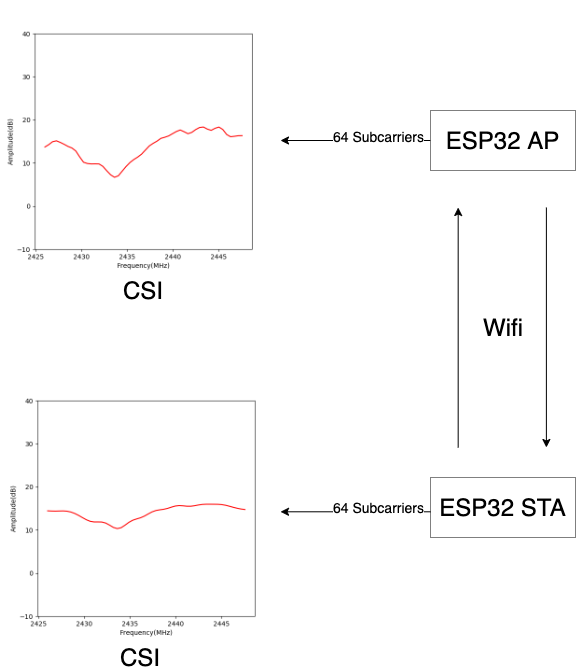
\includegraphics[width=70mm,scale=0.5]{ESP32CSI01.png}}
		\caption{CSI from ESP32s with channel 6.}
		\label{fig:ESP32CSI01}
	\end{figure}
	
	\iffalse
	\subsubsection*{Faraday cage}
	Faraday cage is invented by Michael Faraday in 1836. It is an enclosure to block electromagnetic fields. It is made of conducting material which can affect any radio frequency (e.g. Wi-Fi) to be unable to pass through.
	\fi
	
	\section*{Materials and methods}
	
	\subsection*{Concept}
	\label{concept}
	
	\begin{figure}[htbp]
		
		\centerline{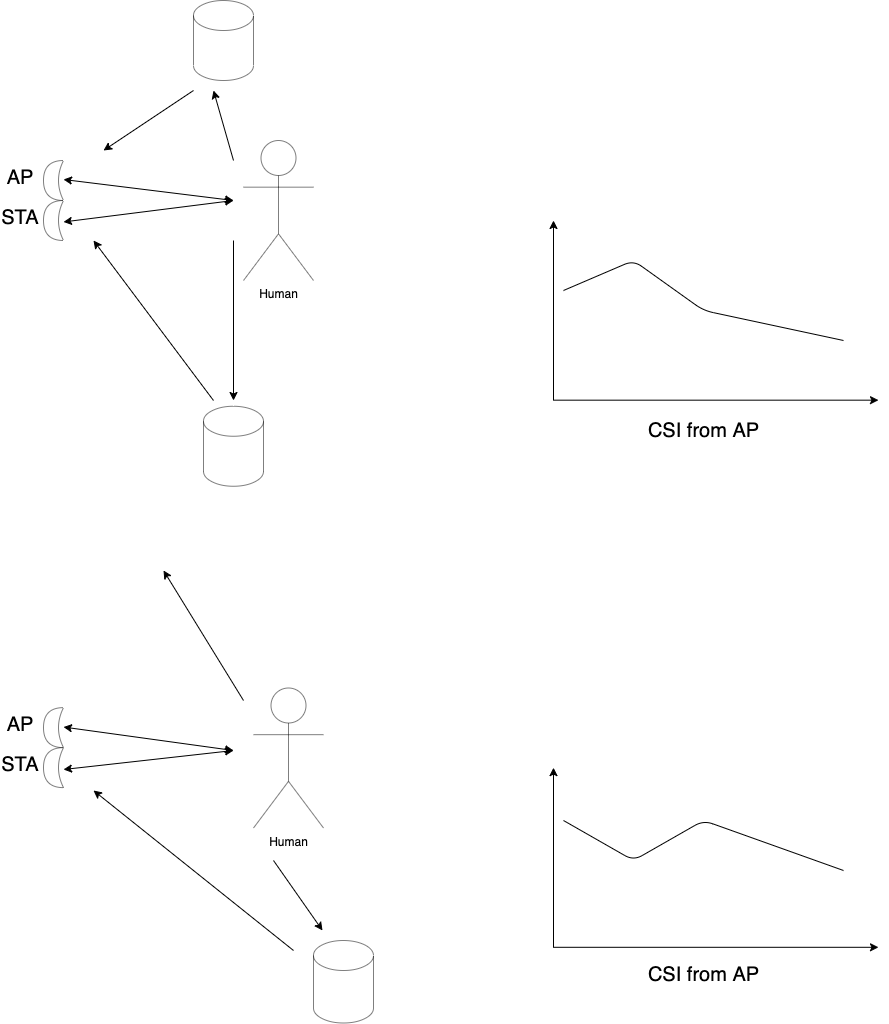
\includegraphics[width=85mm,scale=0.5]{ESP32CSI03.png}}
		\caption{2 different CSIs resulted from corresponding human poses.}
		\label{fig:ESP32CSI02}
	\end{figure}
	
	Other famous proposed works like \cite{wangF} \cite{liuJ} and \cite{hernandezSM} focus on line-of-sight (LOS) in between AP and STA while our work uses 2 directional Wi-Fi antennae and focus on reflection from human body as shown in Fig~\ref{fig:ESP32CSI02} on the left.
	
	
	The reason we named ``Moving Pose Estimation" instead of ``Pose Estimation" is that CSI is not only affected by human body but mainly by overall environment. This means that 2 identical human poses can result obviously different CSIs if the environment around are not exactly the same as shown in Fig~\ref{fig:ESP32CSI02}.
	
	
	So, the definite detection of human standing still in every environment is nearly impossible since the CSI of that situation may be found exactly matched to a CSI of the environment that a big bottle of water placed in front of ESP32.
	In short, if it does not move, we do not know if it is a human.
	
	Meanwhile, the moving pose is totally different because we focus on its change instead. The example of mapping CSI's change to Activity Classification can be found in \cite{chowdhuryTZ} and \cite{zouH}. Our work does likewise but focusing on Pose Estimation instead of Activity Classification.
	
	In different environment, the CSIs are different. But, the corresponding moving pose may affect to the same changing pattern of CSI. This hypothesis is investigated in the upcoming parts.
	
	
	
	
	
	
	All steps of training method is shown in Fig~\ref{fig:TRAINSTEP}. 
	
	
	\begin{figure}[htbp]
		\centerline{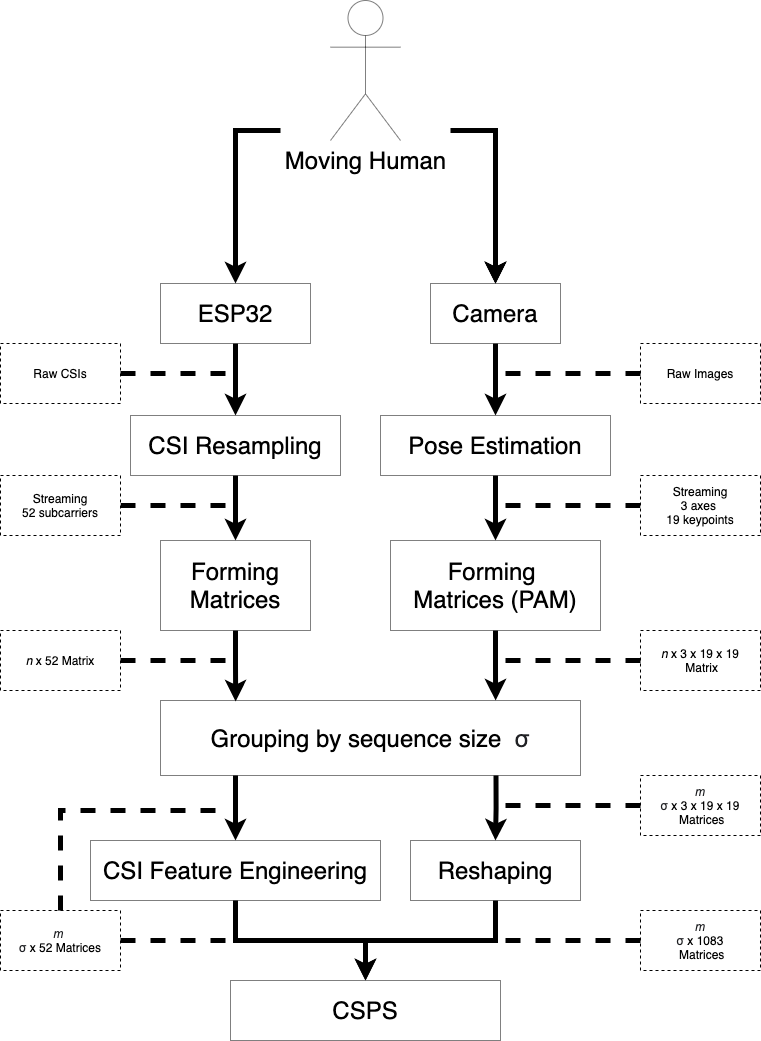
\includegraphics[width=70mm,scale=0.2]{TRAINSTEP06.png}}
		\caption{All steps of training method.}
		\label{fig:TRAINSTEP}
	\end{figure}
	
	
	
	\subsection*{Pre-processing}\label{Processing}
	
	\subsubsection*{CSI Resampling}
	
	
	As mentioned in \nameref{ESP32}, there are 64 subcarriers in CSI data from ESP32 but there are only 52 those are usable while the rest are null. So, we can construst a tensor of $1 \times 52$ to represent each CSI. We are to map CSI from the ESP32 to 3D human pose annotation from a camera. The sampling rate of the camera are set to 30Hz. So, we have 30 human pose annotations for one second. For the ESP32, the sampling rate is originally unpredictable and not constant but it is running around 120Hz. So, we do a process called ``Resampling" to obtain CSI at rate 30Hz in order to synchronize timestamps to each human pose annotation.
	
	An example of CSI Resampling is shown in Fig~\ref{fig:CSIResampling01}. The top graph shows that the the original CSI is logged unstably. The bottom one is to pick a timestamp at rate 30Hz and calculated each with 2 data at the closet timestamps from the original with a simple mathamatical weight equation as in Eq.~\ref{eq:CSIResampling01} in order to predict CSI at timestamp corresponding to each human pose annotation.
	
	\begin{equation}
	\begin{aligned}
	& CSI_{now} = CSI_{before} \\ 
	& + \left(  \frac{ts_{now}-ts_{before}}{ts_{after}-ts_{before}}  \times (CSI_{after}-CSI_{before})   \right),
	\label{eq:CSIResampling01}
	\end{aligned}
	\end{equation}
	where $ts_{now}$, $ts_{before}$, $ts_{after}$ are desired timestamp, timestamp at the closest CSI before the desired timestamp and timestamp at the closest CSI after the desired timestamp respectively. And, $CSI_{now}$, $CSI_{before}$, $CSI_{after}$ are CSI at the desired timestamp, CSI before the desired timestamp and CSI after the desired timestamp respectively.
	
	\begin{figure}[htbp]
		\centerline{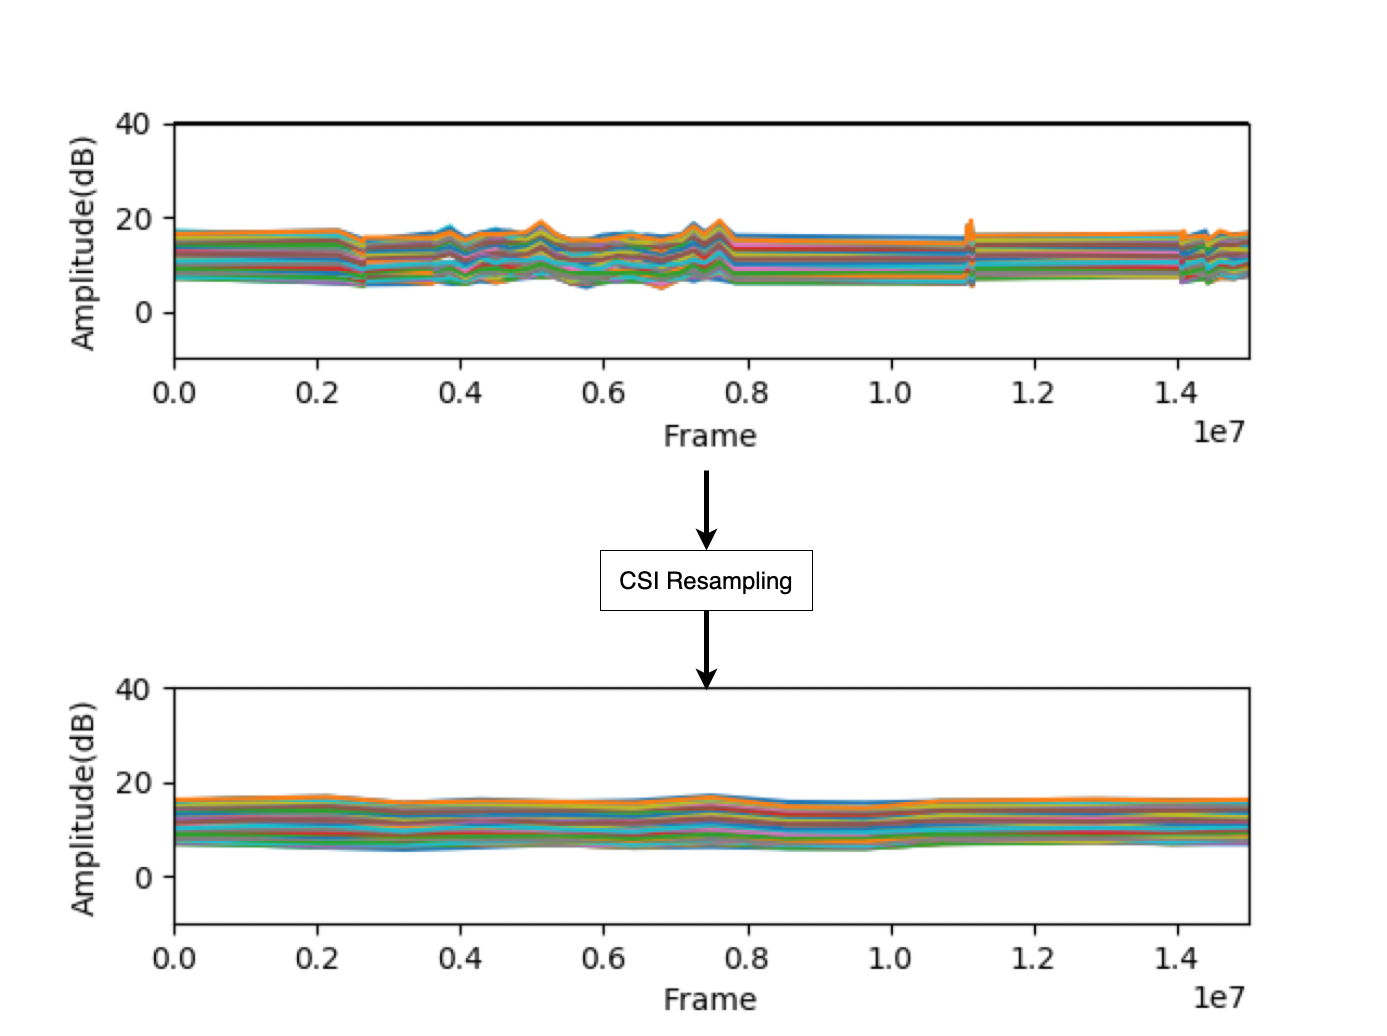
\includegraphics[width=70mm,scale=0.5]{CSIResampling03.png}}
		\caption{An example of CSI resampling.}
		\label{fig:CSIResampling01}
	\end{figure}
	
	Thus, we are able to map each CSI sample to one 3D human pose annotation at the corresponding timestamp.
	
	
	\subsubsection*{Pose Estimation and PAM formation}
	
	
	\begin{figure}[htbp]
		\centerline{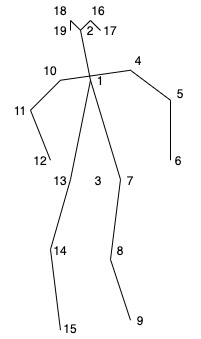
\includegraphics[width=30mm,scale=0.5]{POSEkeypoint02.png}}
		\caption{19 keypoints of human pose.}
		\label{fig:POSEkeypoint}
	\end{figure}
	
	
	
	We use Github-Lw3d$\footnote[1]{https://github.com/Daniil-Osokin/lightweight-human-pose-estimation-3d-demo.pytorch}$ to estimate 3D human pose from videos as stated above. the estimation gives us a $19 \times 3$ matrix for each image. The $19 \times 3$ matrix are used as an annotation where $19$ is for keypoints in human body and $3$ is for 3 axes coordination as shown in Fig~\ref{fig:POSEkeypoint}. But, the annotation can still possess too much independency. Some alignment of keypoints may lead to some impossible pose e.g. hip keypoint found very far from neck keypoint or head keypoint attached to hip keypoint. We assume those poses are not possible for normal human pose. To preserve those constraints, we form a pose adjacent matrix (PAM) from an original $19\times3$ matrix. the PAM is applied for all x, y and z axes. Each are to form their $19\times19$ matrix by the following equations.
	
	\begin{equation}
	x_{i,j}' = \begin{cases}
	x_i-x_j &\text{$i\neq j$}\\
	x_i &\text{$i=j$}\\
	\end{cases}
	\label{eq:xPAM}
	\end{equation},
	\begin{equation}
	y_{i,j}' = \begin{cases}
	y_i-y_j &\text{$i\neq j$}\\
	y_i &\text{$i=j$}\\
	\end{cases}
	\label{eq:yPAM}
	\end{equation}
	and
	\begin{equation}
	z_{i,j}' = \begin{cases}
	z_i-x_j &\text{$i\neq j$}\\
	z_i &\text{$i=j$}\\
	\end{cases}
	\label{eq:zPAM}
	\end{equation}.
	
	The PAM is finally a $3\times19\times19$ matrix created from 3 matrices of $x'$,$y'$ and $z'$ stacked.
	Apparently, one PAM represents one human pose.
	
	
	
	Conclusively, we are making a model by mapping a sequence of $1\times52$ matrix from CSI to each sequence of $ 19 \times 3 \times 3 $ PAM from moving human pose annotation with the corresponding timestamp as shown in Fig~\ref{fig:STEP01}. 
	
	\begin{figure}[htbp]
		\centerline{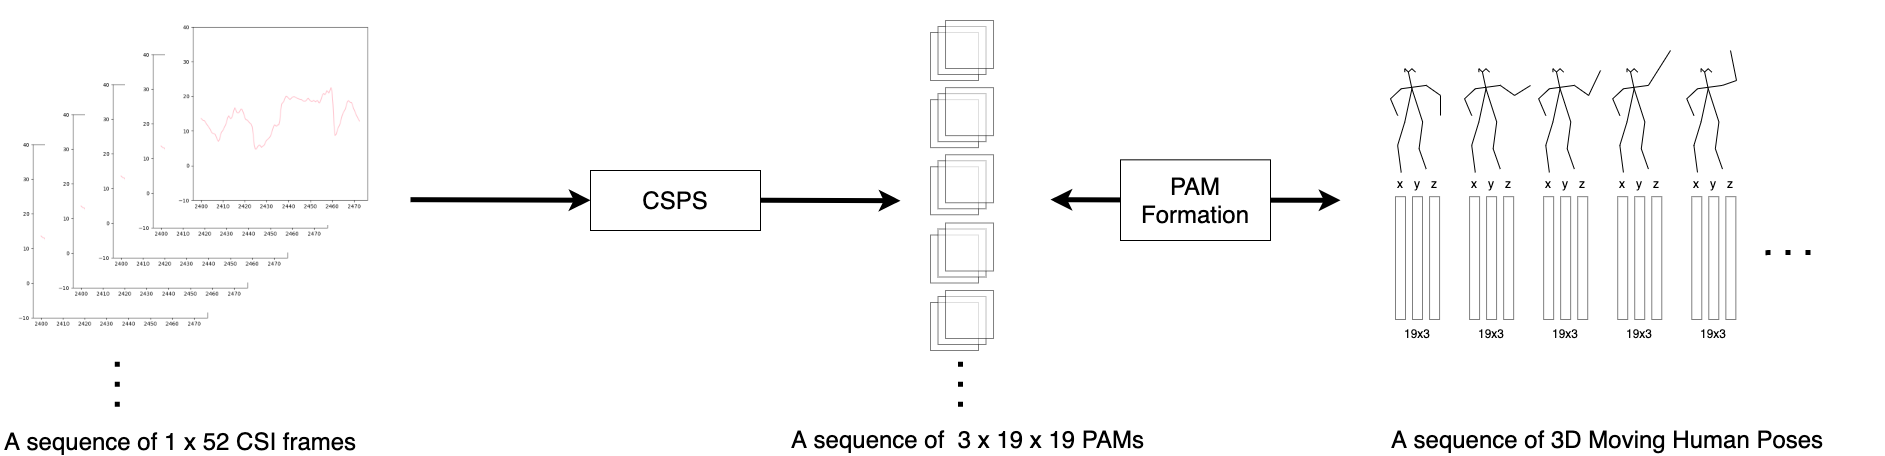
\includegraphics[width=110mm,scale=0.5]{STEP06.png}}
		\caption{A mapping rule from CSI frames to 3D human poses.}
		\label{fig:STEP01}
	\end{figure}
	
	
	
	\subsection*{Processing}
	
	
	\subsubsection*{Mapping CSI and PAM}
	Let $D$ be a set of synchronized pose and CSI data package. Each pair has corresponding timestamp.
	
	\begin{equation}
	D =  {(C_t, P_t), t \in [1, n]},
	\label{eq:Dataset}
	\end{equation} where  $n$ is a number of pairs, $C$ is for CSI data from ESP32, $P$ is for PAM annotation as the ground truth and $t$ is the timestamp index when those 2 were collected.
	
	
	
	\subsubsection*{Grouping By Sequence Size}
	
	Let $\sigma$ be an adjustable window size. $\sigma$ size of $D$ are fed to the model solely. So,  $\sigma \le n$. And, Let $m$ be the number of feeding iteration, $m = \lfloor \frac{n}{\sigma} \rfloor$.
	
	
	The training model swallow $m$ training data as an input, where each is a sequencial set of $(C_t,P_t)$ at a corresponding timestamp with size $\sigma$.
	Let $\Gamma$ be a representation of each sequencial set.
	
	\begin{equation}
	\Gamma =  {(C_u, P_u), u \in [1, \sigma]},
	\label{eq:SubDataset}
	\end{equation}
	where $u$ is the timestamp index when those 2 were collected. Apparently, the size of $\Gamma$ is $m$.
	
	
	As the $\Gamma$ is a sequencial set with size $\sigma$, we assume that Long-short term memory (LSTM) \cite{hochreiterS} is suitable for this type of data.
	
	\iffalse
	\paragraph*{(Optional) CSI Feature Extractor}
	We may extract feature from the CSI before feed it to the model. Or ignore it and feed original CSI to the model directly.
	\fi
	
	\subsubsection*{CSI Feature Engineering}
	As mentioned in \nameref{concept}, CSI ($C$) value implies environment where signal propagating. So, we need to ignore it and focus only on its change in order to universalize the circumstance. It means CSI variousity makes the model not to be applicable in every environment. To solve it, we simply sequentially substract $C_u$  in each $\Gamma$ backward to preserve only how CSI changes over each sequence by the following equation,
	
	
	\begin{equation}
	C_u =  \begin{cases}
	\text{all } 0 &\text{$u = 1$}\\
	C_u - C_{u-1} &\text{$u > 1 $}\\
	\end{cases}, C_u \in \Gamma.
	\label{eq:CSIFeatureEn}
	\end{equation}
	
	\subsubsection*{Forming Network Layer}
	
	\paragraph*{CSI Sequence to Pose Sequence (CSPS)}
	
	The summation of layers is shown in Table~\ref{table:CSPS}.
	It is designed to shape a CSI Sequence ( $\sigma \times 52$ tensor) to a predicted sequence of pose ( $\sigma \times 3\times 19\times 19$ tensor).
	
	\begin{table}[!ht]
		\begin{adjustwidth}{-2.25in}{0in} % Comment out/remove adjustwidth environment if table fits in text column.
			\centering
			\caption{
				{\bf Layers in CSPS.}}
			\begin{tabular}{lll}
				\hline
				Layer (type)       & Output Shape     & Param \# \\ 
				\thickhline
				Bidirectional LSTM & (None, 200)      & 122400   \\
				RepeatVector       & (None, $\sigma$, 200)  & 0        \\
				Bidirectional LSTM & (None, $\sigma$, 200)  & 240800   \\
				TimeDistributed over Dense    & (None, $\sigma$, 1083) & 217683   \\ \hline
			\end{tabular}
			
			\begin{flushleft} 
			\end{flushleft}
			\label{table:CSPS}
		\end{adjustwidth}
	\end{table}
	
	
	We first use Bidirectional LSTM as an encoder layer with the input size of $(\sigma,52)$ to satisfy dimension of sequential $C_u$ in $\Gamma$.
	Then, the repeat vector is added with time $\sigma$ to make the model treat with correct time-step. Afterward, we place a decoder layer with another Bidirectional LSTM. 
	
	Next, we dense the decoder to be $1083$ where can be reshaped into $3\times 19\times 19$ later.
	
	Lastly,  the TimeDistributed layer is used in order to make the model treat the output for each time-step individually.
	
	
	
	% Results and Discussion can be combined.
	\section*{Results}
	
	\subsection*{Data Collection}

	We recruited 10 volunteers to act common movements in front of the devices (a camera and WiFi anntennae) in 3 different environments. The example of the data collection are shown in Fig.~\ref{fig:VIS02} and Fig.~\ref{fig:VIS03} where the top-left is the annotated Pose Estimation, the top-right is a raw video, the vertical center is a raw WiFi CSI and the bottom is a resampled WiFi CSI.
	
	
\begin{figure}[htbp]
	\centerline{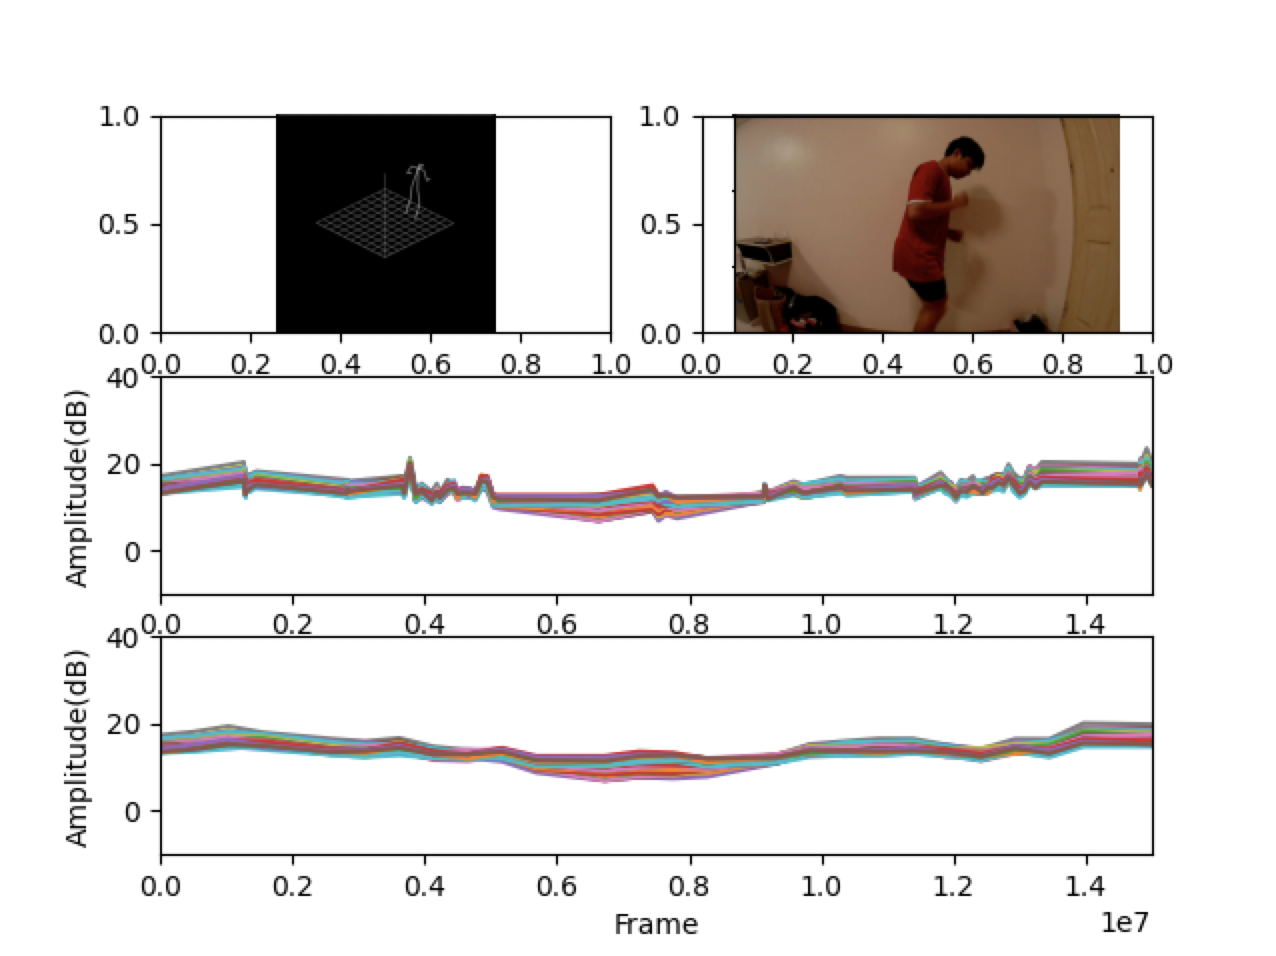
\includegraphics[width=70mm,scale=0.2]{VIS02.png}}
	\caption{An example of data collection.}
	\label{fig:VIS02}
\end{figure}
\begin{figure}[htbp]
	\centerline{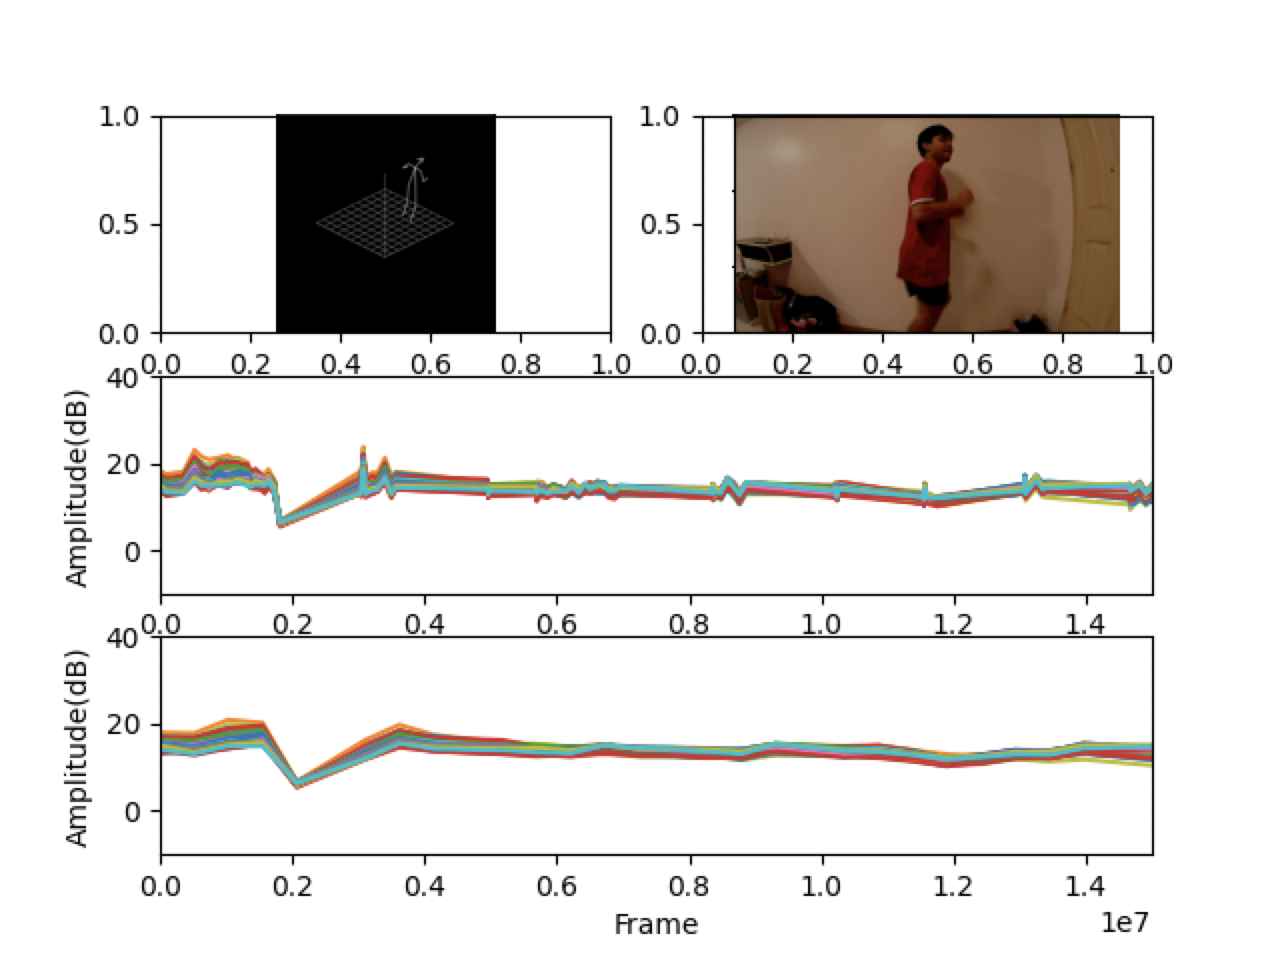
\includegraphics[width=70mm,scale=0.2]{VIS03.png}}
	\caption{An example of data collection.}
	\label{fig:VIS03}
\end{figure}


	The whole data collected is an hour of videos and WiFi CSI which worths 180,000 frames for 30 fps rate. The ratio of dataset for training and testing is 80/20.
	
	
	\subsection*{Error Metric}
	
	
	Percentage of Correct Keypoint (PCK) is widely used to evaluate the performance of human pose estimation according to \cite{wangF}.
	
	\begin{equation}
	\begin{aligned}
	PCK_i@a = \frac{1}{N} \sum_{i=1}^{N}
	I(
	\frac{\mid \mid  pd_i \text{ - } gt_i \mid \mid^2_2}{\sqrt{rh^2+lh^2}}  \le a ),
	\label{eq:PCK}
	\end{aligned}
	\end{equation}
	
	
	where $I$(·) is a binary indicator that outputs 1 while true and 0 while false, 
	$N$ is the number of frames and $i$ is the index of keypoints that $i \in {1, 2, ..., 19}$. The $rh$ and
	$lh$ are for the positions of the right shoulder and the left hip from the ground truth, respectively.
	So, the ${\sqrt{rh^2+lh^2}}$ is  considered as the length of the upper limb from the ground truth, which is used to normalize the prediction error length
	$ \mid \mid pd_i \text{ - } gt_i \mid \mid _2^2$, and $pd_i$ and $gt_i$ are coordinates of prediction and ground-truth at the keypoint $i$ respectively.
	
	
	
	\subsection*{Experimental Result}
	\label{result}
	All steps of testing method is shown in Fig~\ref{fig:TESTSTEP}. 
	
	\begin{figure}[htbp]
		\centerline{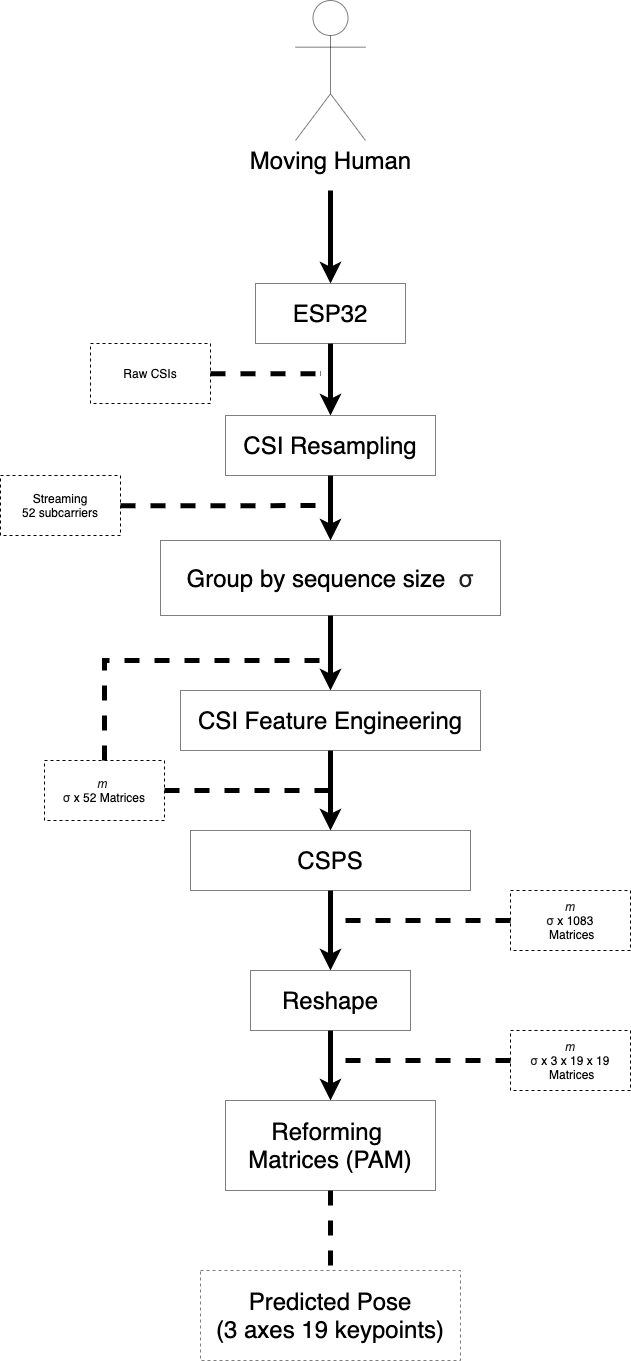
\includegraphics[width=60mm,scale=0.2]{TESTSTEP06.png}}
		\caption{All steps of testing method.}
		\label{fig:TESTSTEP}
	\end{figure}
	
	
	
	
	An evaluation is achieved   by the algorithm written in Python 3.8. The code is available on 	Github$\footnote[1]{https://github.com/rtmtree/CSPS}$.
	An environment under the evaluation is MacBook Pro 2016, 2.6 GHz i7 processor, 16 GB of RAM.
	
		The visual examples are shown in \ref{fig:PREDANNO01} and \ref{fig:PREDANNO02} where the top-left is the predicted pose, the top-right is the annotated pose and bottom is the resampled WiFi CSI that the prediction took as an input. Note that the predicted  and the annotated pose are actually moving in range of $\sigma$.
	
	
	\begin{figure}[htbp]
		\centerline{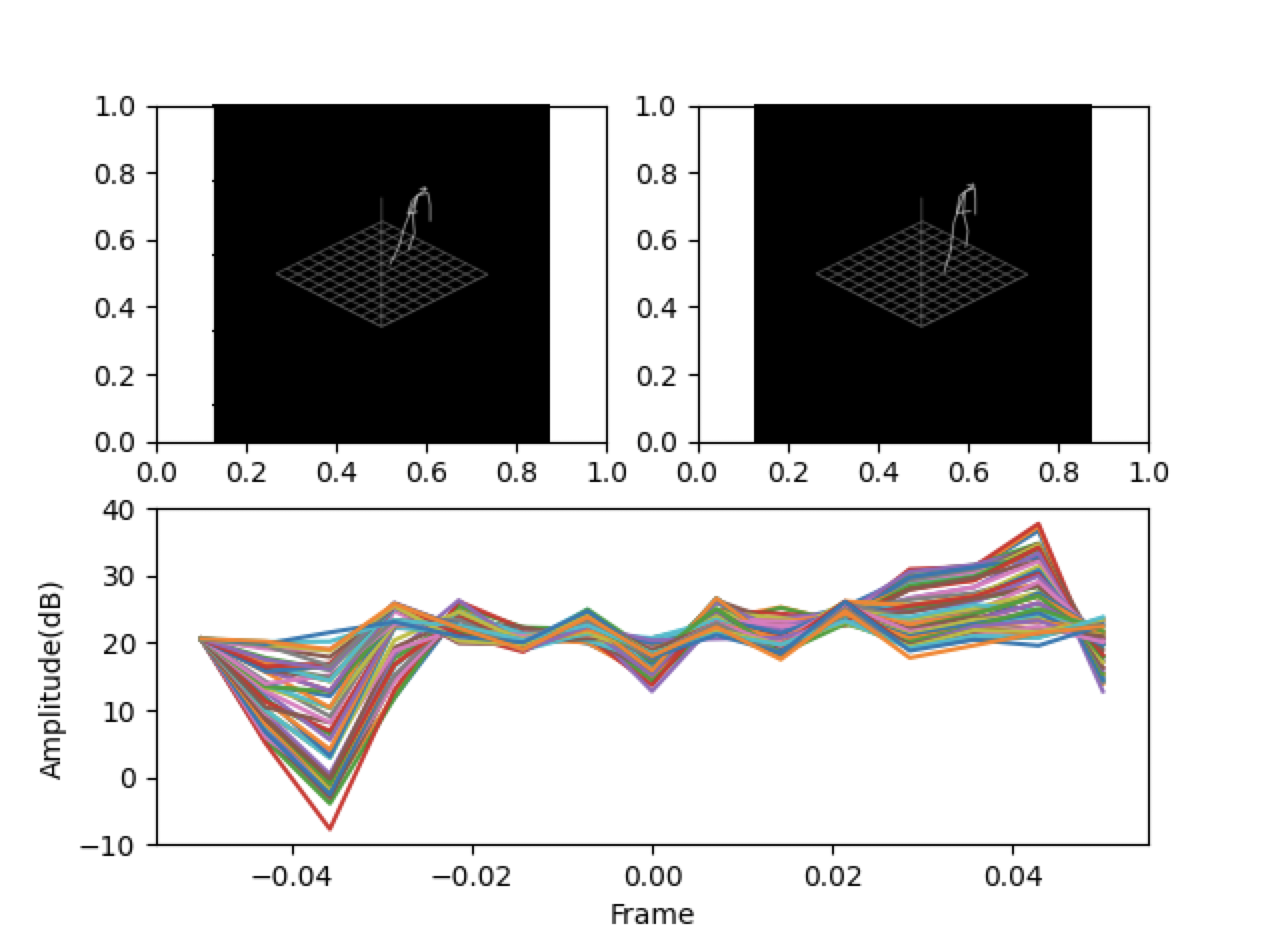
\includegraphics[width=100mm,scale=0.2]{PREDANNO01.png}}
		\caption{An example of comparison between predicted pose and annotated pose when $\sigma=15$.}
		\label{fig:PREDANNO01}
	\end{figure}
	\begin{figure}[htbp]
		\centerline{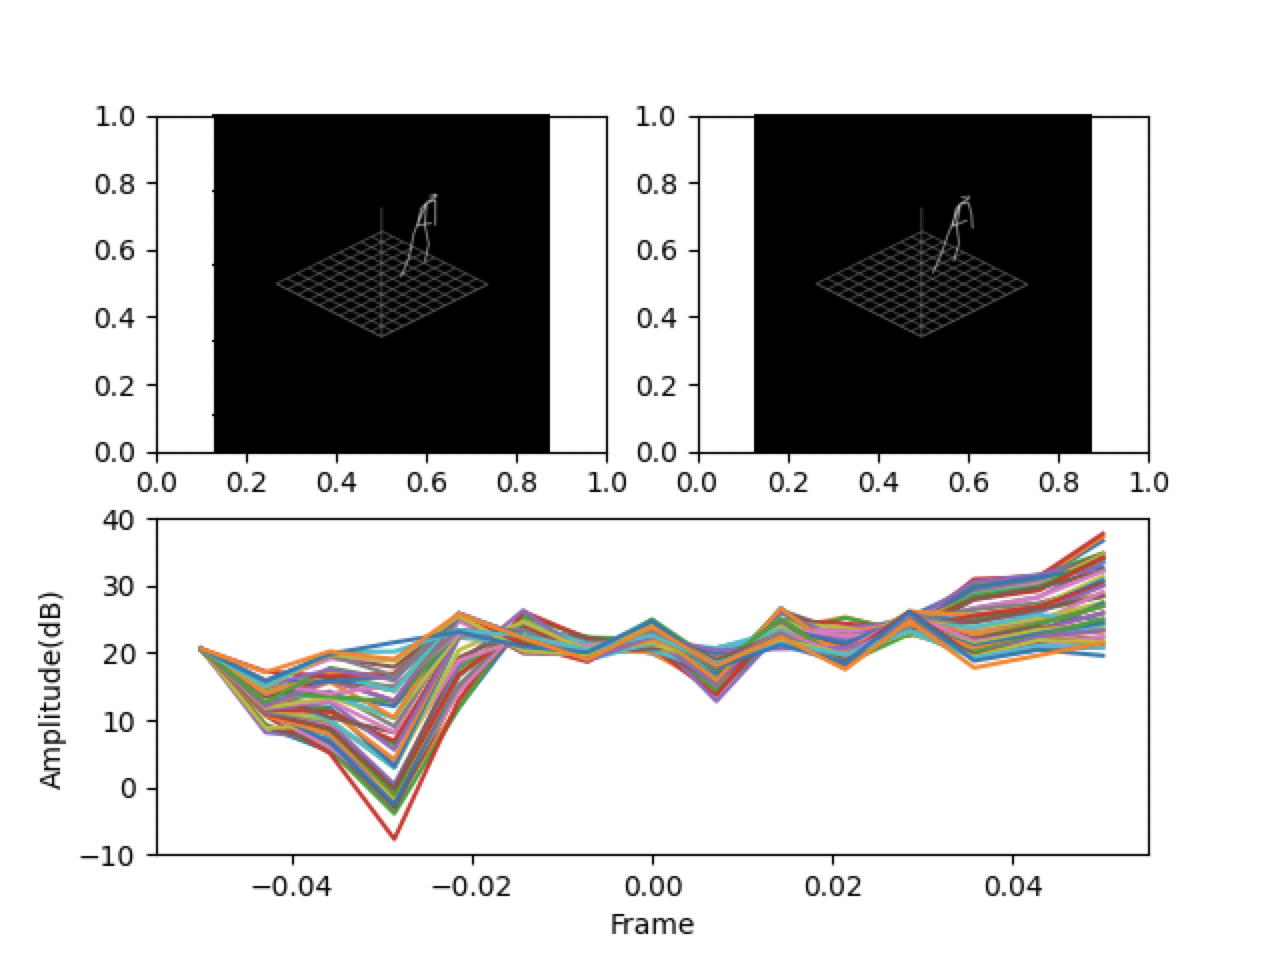
\includegraphics[width=100mm,scale=0.2]{PREDANNO02.png}}
		\caption{An example of comparison between predicted pose and annotated pose when $\sigma=15$.}
		\label{fig:PREDANNO02}
	\end{figure}
	
	
	As parameters stated in the previous sections, we demostrated the prediction by the followings.
	
	Table~\ref{table:PCKsigma15}, Table~\ref{table:PCKsigma20}, Table~\ref{table:PCKsigma30} and  Table~\ref{table:PCKsigma40} show the estimation performance of 19 body keypoints in PCK when $\sigma=15$, $\sigma=20$, $\sigma=30$ and $\sigma=40$ respectively.


	
\begin{table}[!ht]
\begin{adjustwidth}{-2.25in}{0in} % Comment out/remove adjustwidth environment if table fits in text column.
	\centering
	\caption{
		{\bf Table of PCK when $\sigma=15$.}}
	\begin{tabular}{|l|l|l|l|l|l|l|l|}
		\hline
		Order & Keypoint & PCK@5 & PCK@10 & PCK@20 & PCK@30 & PCK@40 & PCK@50 \\ \thickhline
		1     &  Neck       & 0.7553      &  0.8993      &  0.9443      & 0.9590       &   0.9717     & 0.98100       \\ \hline
		2     &  Nose        & 0.0383      &  0.4885      &  0.9038      &  0.9498      &   0.9649     & 0.9724        \\ \hline
		3     &  Hip (Invisible)        & 0.7626      &  0.9033      &  0.9437      & 0.9583       &  0.9688      & 0.9796       \\ \hline
		4     &  L. Shoulder         & 0.6502      & 0.8436       & 0.9426       & 0.9665       &  0.9766      & 0.9828       \\ \hline
		5     &  L. Elbow        & 0.6055      &  0.7786      &  0.9001      &  0.9482      &  0.9681      &  0.9772      \\ \hline
		6     &  L. Wrist        & 0.3149      &  0.5845      &  0.8135      &  0.9013      &  0.9415      &  0.9625      \\ \hline
		7     &  L. Hip        &  0.6866     &   0.8678     &  0.9485      & 0.9653       &  0.9765      &  0.9862      \\ \hline
		8     &  L. Knee         & 0.5571      &  0.7794      &  0.9194      & 0.9587       &  0.9747      &  0.9837      \\ \hline
		9     &  L. Ankle         &  0.4132     &  0.6572      &   0.8617     &   0.9292     &  0.9583      & 0.9740       \\ \hline
		10    &  R. Shoulder        & 0.6419      &  0.8407      &  0.9364      & 0.9527       & 0.9618       &  0.9709      \\ \hline
		11    &  R. Elbow        & 0.5966      &  0.7596      &  0.8854      &  0.9321      &  0.9532      &  0.9632      \\ \hline
		12    &  R. Wrist        & 0.3031      &  0.5936      &  0.8204      &  0.9132      &  0.9386      &  0.9496      \\ \hline
		13    &  R. Hip        & 0.6895      &   0.8690     &  0.9404      &  0.9547      &    0.9663    &   0.9778     \\ \hline
		14    &  R. Knee        &  0.5626     &  0.7750      &  0.9169      &  0.9493      &   0.9631     &  0.9753      \\ \hline
		15    &  R. Ankle        & 0.4370  &   0.6611     &   0.8627     &  0.9301      &    0.9552    &   0.9711     \\ \hline
		16    &  L. Eye        & 0.0279      &  0.4281      &  0.8955      & 0.9493       &  0.9638      &  0.9740      \\ \hline
		17    &  L. Ear        &  0.0677     &  0.6447      &  0.9250     & 0.9571       &   0.9709     &  0.9830      \\ \hline
		18    &  R. Eye        & 0.0204      &  0.2476      &  0.8729      & 0.9476       &  0.9617      & 0.9706       \\ \hline
		19    &  R. Ear        & 0.0326      &  0.5010      &  0.9182      &  0.9527      &  0.9638      &  0.9729      \\ \hline
		Avg    &  &  0.4296        & 0.6907      & 0.9027       &  0.9461      &   0.9631     &   0.9741             \\ \hline
	\end{tabular}
	\label{table:PCKsigma15}
\end{adjustwidth}
\end{table}

\begin{table}[!ht]
	\begin{adjustwidth}{-2.25in}{0in} % Comment out/remove adjustwidth environment if table fits in text column.
		\centering
		\caption{
			{\bf Table of PCK when $\sigma=20$.}}
		\begin{tabular}{|l|l|l|l|l|l|l|l|}
			\hline
			Order & Keypoint & PCK@5 & PCK@10 & PCK@20 & PCK@30 & PCK@40 & PCK@50 \\ \thickhline
			1     &  Neck       &0.7698 & 0.9026 & 0.9511 & 0.9658 & 0.9748 & 0.9816       \\ \hline
			2     &  Nose        &  0.6612 & 0.8463 & 0.9452 & 0.9625 & 0.9710 & 0.9771        \\ \hline
			3     &  Hip (Invisible)        & 0.7601 & 0.9025 & 0.9522 & 0.9671 & 0.9750 & 0.9815       \\ \hline
			4     &  L. Shoulder         & 0.6680 & 0.8563 & 0.9483 & 0.9717 & 0.9810 & 0.9864       \\ \hline
			5     &  L. Elbow        & 0.6056 & 0.7845 & 0.9051 & 0.9571 & 0.9753 & 0.9827      \\ \hline
			6     &  L. Wrist        & 0.3196 & 0.5872 & 0.8178 & 0.9027 & 0.9400 & 0.9614      \\ \hline
			7     &  L. Hip        &  0.6827 & 0.8711 & 0.9508 & 0.9700 & 0.9805 & 0.9873      \\ \hline
			8     &  L. Knee         & 0.5637 & 0.7773 & 0.9169 & 0.9584 & 0.9767 & 0.9844      \\ \hline
			9     &  L. Ankle         &  0.4373 & 0.6639 & 0.8598 & 0.9269 & 0.9571 & 0.9740       \\ \hline
			10    &  R. Shoulder        & 0.6589 & 0.8506 & 0.9444 & 0.9618 & 0.9705 & 0.9757      \\ \hline
			11    &  R. Elbow        & 0.5979 & 0.7650 & 0.8904 & 0.9394 & 0.9636 & 0.9725      \\ \hline
			12    &  R. Wrist        & 0.2985 & 0.5901 & 0.8169 & 0.9148 & 0.9465 & 0.9593      \\ \hline
			13    &  R. Hip        & 0.6917 & 0.8765 & 0.9501 & 0.9637 & 0.9728 & 0.9800     \\ \hline
			14    &  R. Knee        &  0.5676 & 0.7853 & 0.9259 & 0.9561 & 0.9682 & 0.9774       \\ \hline
			15    &  R. Ankle        & 0.4532 & 0.6723 & 0.8734 & 0.9385 & 0.9600 & 0.9730     \\ \hline
			16    &  L. Eye        & 
			0.6721 & 0.8515 & 0.9455 & 0.9632 & 0.9723 & 0.9785      \\ \hline
			17    &  L. Ear        &  0.7239 & 0.8810 & 0.9482 & 0.9660 & 0.9762 & 0.9843      \\ \hline
			18    &  R. Eye        & 0.6658 & 0.8477 & 0.9459 & 0.9626 & 0.9706 & 0.9764       \\ \hline
			19    &  R. Ear        & 0.7091 & 0.8810 & 0.9492 & 0.9631 & 0.9715 & 0.9775      \\ \hline
			Avg    &  &  0.6056 & 0.7996 & 0.9177 & 0.9532 & 0.9686 & 0.9774             \\ \hline
		\end{tabular}
		\label{table:PCKsigma20}
	\end{adjustwidth}
\end{table}
	
\begin{table}[!ht]
	\begin{adjustwidth}{-2.25in}{0in} % Comment out/remove adjustwidth environment if table fits in text column.
		\centering
		\caption{
			{\bf Table of PCK when $\sigma=30$.}}
		\begin{tabular}{|l|l|l|l|l|l|l|l|}
			\hline
			Order & Keypoint & PCK@5 & PCK@10 & PCK@20 & PCK@30 & PCK@40 & PCK@50 \\ \thickhline
			1     &  Neck    & 0.7580 & 0.8866 & 0.9373 & 0.9547 & 0.9654 & 0.9748      \\ \hline
			2     &  Nose     & 0.6631 & 0.8315 & 0.9315 & 0.9512 & 0.9620 & 0.9688       \\ \hline
			3     &  Hip (Invisible)     & 0.7507 & 0.8873 & 0.9390 & 0.9561 & 0.9659 & 0.9759      \\ \hline
			4     &  L. Shoulder      & 0.6680 & 0.8418 & 0.9300 & 0.9564 & 0.9703 & 0.9785      \\ \hline
			5     &  L. Elbow      & 0.6143 & 0.7760 & 0.8943 & 0.9426 & 0.9644 & 0.9740     \\ \hline
			6     &  L. Wrist     & 0.3116 & 0.5755 & 0.8023 & 0.8888 & 0.9316 & 0.9541      \\ \hline
			7     &  L. Hip     & 0.6828 & 0.8597 & 0.9366 & 0.9590 & 0.9694 & 0.9806      \\ \hline
			8     &  L. Knee      & 0.5584 & 0.7719 & 0.9096 & 0.9492 & 0.9669 & 0.9778      \\ \hline
			9     &  L. Ankle      & 0.4332 & 0.6620 & 0.8575 & 0.9215 & 0.9498 & 0.9665      \\ \hline
			10    &  R. Shoulder     & 0.6719 & 0.8453 & 0.9322 & 0.9495 & 0.9613 & 0.9696      \\ \hline
			11    &  R. Elbow     & 0.6255 & 0.7772 & 0.8859 & 0.9331 & 0.9548 & 0.9653      \\ \hline
			12    &  R. Wrist     & 0.3134 & 0.6091 & 0.8155 & 0.9038 & 0.9336 & 0.9477      \\ \hline
			13    &  R. Hip     & 0.6974 & 0.8637 & 0.9361 & 0.9536 & 0.9673 & 0.9770      \\ \hline
			14    &  R. Knee     & 0.5828 & 0.7854 & 0.9127 & 0.9455 & 0.9617 & 0.9730      \\ \hline
			15    &  R. Ankle     & 0.4678 & 0.6847 & 0.8693 & 0.9303 & 0.9523 & 0.9671      \\ \hline
			16    &  L. Eye     & 0.6712 & 0.8364 & 0.9316 & 0.9518 & 0.9629 & 0.9704      \\ \hline
			17    &  L. Ear     & 0.7145 & 0.8664 & 0.9337 & 0.9544 & 0.9660 & 0.9767      \\ \hline
			18    &  R. Eye     & 0.6648 & 0.8322 & 0.9322 & 0.9508 & 0.9612 & 0.9685      \\ \hline
			19    &  R. Ear     & 0.7068 & 0.8645 & 0.9350 & 0.9522 & 0.9622 & 0.9709      \\ \hline
			Avg  &  &    0.6082 & 0.7925 & 0.9064 & 0.9423 & 0.9594 & 0.9704        \\ \hline
		\end{tabular}
		\label{table:PCKsigma30}
	\end{adjustwidth}
\end{table}

\begin{table}[!ht]
	\begin{adjustwidth}{-2.25in}{0in} % Comment out/remove adjustwidth environment if table fits in text column.
		\centering
		\caption{
			{\bf Table of PCK when $\sigma=40$.}}
		\begin{tabular}{|l|l|l|l|l|l|l|l|}
			\hline
			Order & Keypoint & PCK@5 & PCK@10 & PCK@20 & PCK@30 & PCK@40 & PCK@50 \\ \thickhline
			1     &  Neck    & 0.7480 & 0.8822 & 0.9339 & 0.9519 & 0.9658 & 0.9746      \\ \hline
			2     &  Nose     & 0.6546 & 0.8270 & 0.9273 & 0.9484 & 0.9614 & 0.9707       \\ \hline
			3     &  Hip (Invisible)     & 0.7435 & 0.8832 & 0.9361 & 0.9542 & 0.9675 & 0.9780      \\ \hline
			4     &  L. Shoulder      & 0.6703 & 0.8406 & 0.9263 & 0.9529 & 0.9683 & 0.9781      \\ \hline
			5     &  L. Elbow      & 0.6156 & 0.7802 & 0.8968 & 0.9398 & 0.9618 & 0.9727     \\ \hline
			6     &  L. Wrist     & 0.3259 & 0.5890 & 0.8076 & 0.8939 & 0.9330 & 0.9551      \\ \hline
			7     &  L. Hip     & 0.6649 & 0.8491 & 0.9339 & 0.9556 & 0.9684 & 0.9805      \\ \hline
			8     &  L. Knee      & 0.5393 & 0.7585 & 0.9044 & 0.9471 & 0.9663 & 0.9765      \\ \hline
			9     &  L. Ankle      & 0.4188 & 0.6476 & 0.8437 & 0.9162 & 0.9485 & 0.9664      \\ \hline
			10    &  R. Shoulder     & 0.6654 & 0.8353 & 0.9264 & 0.9473 & 0.9605 & 0.9703      \\ \hline
			11    &  R. Elbow     & 0.6245 & 0.7786 & 0.8791 & 0.9272 & 0.9525 & 0.9656      \\ \hline
			12    &  R. Wrist     & 0.3115 & 0.5966 & 0.8159 & 0.9057 & 0.9340 & 0.9481      \\ \hline
			13    &  R. Hip     & 0.6894 & 0.8598 & 0.9328 & 0.9525 & 0.9683 & 0.9785      \\ \hline
			14    &  R. Knee     & 0.5753 & 0.7826 & 0.9090 & 0.9448 & 0.9621 & 0.9737      \\ \hline
			15    &  R. Ankle     & 0.4619 & 0.6786 & 0.8663 & 0.9281 & 0.9521 & 0.9668      \\ \hline
			16    &  L. Eye     & 0.6629 & 0.8317 & 0.9274 & 0.9493 & 0.9630 & 0.9723      \\ \hline
			17    &  L. Ear     & 0.7088 & 0.8610 & 0.9302 & 0.9521 & 0.9678 & 0.9767      \\ \hline
			18    &  R. Eye     & 0.6579 & 0.8285 & 0.9269 & 0.9483 & 0.9608 & 0.9701      \\ \hline
			19    &  R. Ear     & 0.6950 & 0.8608 & 0.9312 & 0.9491 & 0.9629 & 0.9715      \\ \hline
			Avg  &  &    0.6018 & 0.7880 & 0.9029 & 0.9402 & 0.9592 & 0.9709        \\ \hline
		\end{tabular}
		\label{table:PCKsigma40}
	\end{adjustwidth}
\end{table}



\section*{Discussion}

\subsection*{WiFi Antennae and Camera Installation}

	The Installation of WiFi antennae and camera can affect tremendously in data. We used a hanger and a camera stand to lock the fixed installation in both training and testing process as shown in Fig~\ref{fig:ANTENSETUP01}.
	2 antennae are connecting to ESP32s and to the PC afterward.
	\begin{figure}[htbp]
	\centerline{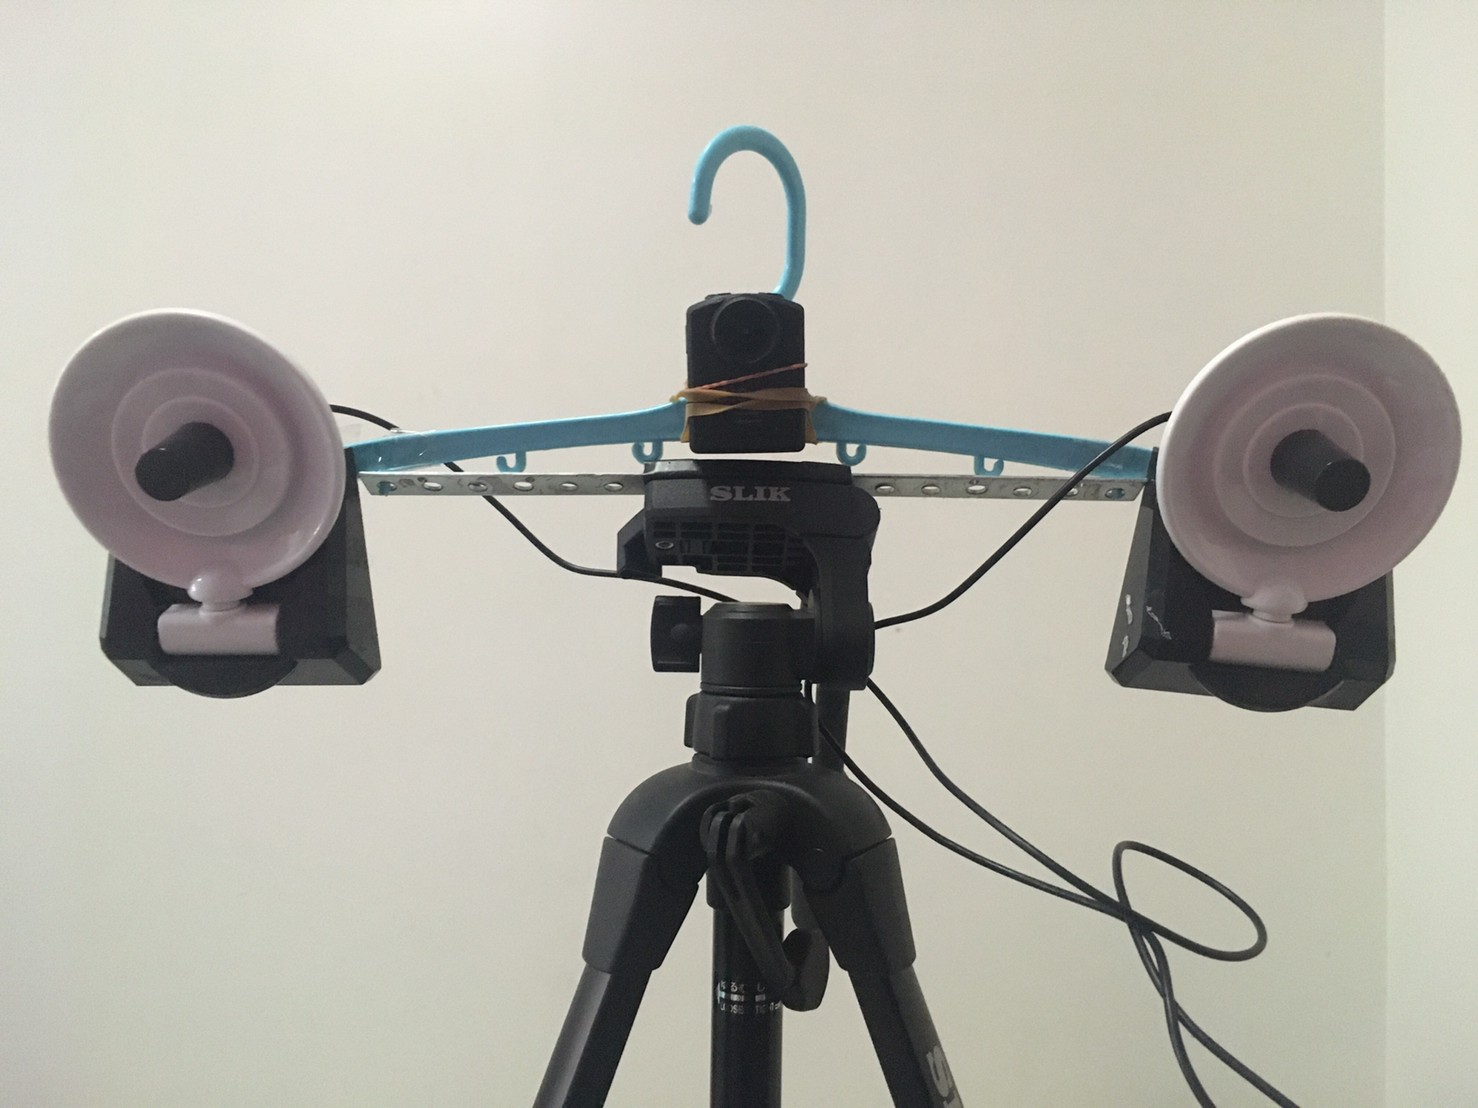
\includegraphics[width=40mm,scale=0.2]{ANTENSETUP01.jpg}}
	\caption{WiFi Antennae and Camera Setup.}
	\label{fig:ANTENSETUP01}
\end{figure}





\subsection*{CSI Extraction Method}

There are many soluions for extracting WiFi CSI from the ESP as mentioned in \nameref{ESP32}. This paper picked the solution from ESP32-CSI-Tool$\footnote[1]{https://github.com/StevenMHernandez/ESP32-CSI-Tool}$ since it is considerably well-written and simple to organize. To change the method of extracting WiFi CSI would affect the result significantly.






\subsection*{Multiple Person Pose Estimation}

The model does the mapping rule from WiFi CSI with a specific dimension to human pose matrix. So, it is able to only detect single person pose in a range. The annotations originally result all human poses from the videos but we decided to crop it to be only one person in order to increase the precision. If we do training with multiple person pose data instead, we believe the result will be well but the more huge data collection is also needed.

\subsection*{Human speed of moving to $\sigma$}

As the Table~\ref{table:PCKsigma15}, Table~\ref{table:PCKsigma20}, Table~\ref{table:PCKsigma30} and  Table~\ref{table:PCKsigma40} show the difference of quality by different value of $\sigma$, the fine-tuning says that $\sigma=15$ result the best. This implies length of $15$ frames can represent a specific pattern of move best for the used dataset. So, the volunteer who recorded movement in the datasent perform a move slower, $\sigma$ should be extended to cover the proper time peroid of the movement pattern.


 	\section*{Conclusion}

	Currently, there are many issues on security occuring in all ranges of human especially in elderlies and those who are not capable to live solely. To solve those, issues on privacy usually comes instead e.g. recording videos for preventing accident in a house, monitoring of people in a room. Many people do not feel very comfortable on these. So, we seek a solution where we can monitor those activity without a camera needed. 
	
	After having a research, we discoverd that a variation in WiFi called WiFi CSI can tell whether the area is having an activity or moving objects. Moreoever, \cite{chowdhuryTZ}, \cite{zouH} and many other works had been done very well on detecting even what kind of activities is happening in the area. We do not believe that this is the limitation of WiFi CSI. In order to solve the above problem and prove if WiFi CSI is precise enough, we tried to overcome this by extracting a deeper information like Pose Estimation from it. 
	
	We controlled environments and enhanced WiFi Antennae stability as much as possible then mapped it to the Pose annotated by an existing Image to Pose Model. The result was very poor since the WiFi CSI is very vague. It penetrates through most of the things. We learned from \cite{bib20} that WiFi CSI value does not matter than its change. The works used Long-short term memory (LSTM), a neural network where focusing on sequence of the data, and obtained a very good result. 
	
	
	We applied the idea of LSTM on our work which made it not Pose Estimation but Moving Pose Estimation instead and obtained a lot better result. Then, we adjusted the model to be suite to our type of data and did fine-tuning for the frame size to be fit the most for normal human speed of moving. So, This paper proposed a model of mapping rule that can takes a sequence of WiFi circumstance as an input and return an according sequence of human pose as an output. The work can help people to monitor activity of elderlies and people who are in need of caring. Moreover as a camera is not needed, we can reduce an issue on privacy infringement and also cure the data size normal camera conducted as WiFi CSI is carrying much lower data size.
	The result of various fine-tuned environments and parammeters is acceptable and shown in \nameref{result}.
	

	\section*{Acknowledgments}
	We thank to Sirindhorn International Institute of Technology for providing technical environment and supportive information.
	
	
	
	\nolinenumbers
	
	% Either type in your references using
	% \begin{thebibliography}{}
	% \bibitem{}
	% Text
	% \end{thebibliography}
	%
	% or
	%
	% Compile your BiBTeX database using our plos2015.bst
	% style file and paste the contents of your .bbl file
	% here. See http://journals.plos.org/plosone/s/latex for 
	% step-by-step instructions.
	% 
	\begin{thebibliography}{10}
		
		\bibitem{bib1}
		Conant GC, Wolfe KH.
		\newblock {{T}urning a hobby into a job: how duplicated genes find new
			functions}.
		\newblock Nat Rev Genet. 2008 Dec;9(12):938--950.
		
		\bibitem{bib2}
		Ohno S.
		\newblock Evolution by gene duplication.
		\newblock London: George Alien \& Unwin Ltd. Berlin, Heidelberg and New York:
		Springer-Verlag.; 1970.
		
		\bibitem{bib3}
		Magwire MM, Bayer F, Webster CL, Cao C, Jiggins FM.
		\newblock {{S}uccessive increases in the resistance of {D}rosophila to viral
			infection through a transposon insertion followed by a {D}uplication}.
		\newblock PLoS Genet. 2011 Oct;7(10):e1002337.
		
		
		
		
		\bibitem{bib4}
		Osokin D.
		\newblock {{R}eal-time 2D Multi-Person Pose Estimation on CPU: Lightweight OpenPose}.
		\newblock arXiv:1811.12004 [cs.CV]. 2018 Nov;18.
		
		\bibitem{bib5}
		Mehta D, Sotnychenko O, Mueller F, Xu W, Sridhar S, Pons-Moll G, Theobalt C.
		\newblock {{S}ingle-Shot Multi-Person 3D Pose Estimation From Monocular RGB}.
		\newblock arXiv:1712.03453 [cs.CV]. 2018 Aug;28.
		
		
		\bibitem{wangF}
		Wang F, Panev S, Ziyi D, Han J, Huang D.
		\newblock {{C}an WiFi Estimate Person Pose?}.
		\newblock arXiv:1904.00277 [cs.CV]. 2019 Apr;2.
		
		
		
		\bibitem{liuJ}
		Liu J, Liu H, Chen Y, Wang Y, Wang C.
		\newblock {{W}ireless Sensing for Human Activity: A Survey}.
		\newblock IEEE COMMUNICATIONS SURVEYS \& TUTORIALS, VOL. 22, NO. 3, THIRD QUARTER 2020.
		
		\bibitem{chowdhuryTZ}
		Chowdhury TZ, Leung C, Miao CY.
		\newblock {{W}iHACS: Leveraging WiFi for Human Activity Classification using OFDM Subcarriers’ correlation}.
		\newblock IEEE, GlobalSIP 2017.
		
		
		\bibitem{bib9}
		Guo L, Wang L, Liu J, Zhou W, Lu B.
		\newblock {{H}uAc: Human Activity Recognition Using Crowdsourced WiFi
			Signals and Skeleton Data}.
		\newblock Wireless Communications and Mobile Computing
		Volume 2018, Article ID 6163475.
		
		
		
		\bibitem{bib10}
		Wang F, Feng J, Zhao Y, Xiaobin Zhang, Zhang S.
		\newblock {{J}oint Activity Recognition and Indoor
			Localization with WiFi Fingerprints}.
		\newblock arXiv:1904.04964 [cs.CV]. 2019 Jul;18.
		
		
		\bibitem{bib11}
		Al-qaness MAA, Li F, Ma X, Zhang Y, Liu G.
		\newblock {Device-Free Indoor Activity Recognition System}.
		\newblock Appl. Sci. 2016, 6, 329; doi:10.3390.
		
		\bibitem{bib12}
		Wang W, Liu AX, Shahzad M, Ling K, Lu S.
		\newblock {{D}evice-free Human Activity Recognition Using Commercial WiFi Devices}.
		\newblock  IEEE Journal
		on Selected Areas in Communications. DOI 10.1109/JSAC.2017.2679658.
		
		\bibitem{bib13}
		Zhao T, Li F, Tian P.
		\newblock {{A} Deep-Learning Method for Device Activity Detection in mMTC Under Imperfect CSI Based on Variational-Autoencoder}.
		\newblock IEEE TRANSACTIONS ON VEHICULAR TECHNOLOGY, VOL. 69, NO. 7, JULY 2020.
		
		\bibitem{bib14}
		Liu J, Teng G, Hong F.
		\newblock {{H}uman Activity Sensing with Wireless Signals: A Survey}.
		\newblock Sensors 2020, 20, 1210; doi:10.3390/s20041210.
		
		\bibitem{bib15}
		Yousefi S, Narui H, Dayal S, Ermon S, Valaee S.
		\newblock {{A} Survey on Behaviour Recognition Using WiFi Channel State Information}.
		\newblock arXiv:1708.07129 [cs.AI]. 2017 Aug;23.
		
		\bibitem{bib16}
		Chen Z, Zhang L, Jiang C, Cao Z, Cui W.
		\newblock {{W}iFi CSI Based Passive Human Activity Recognition Using Attention Based BLSTM}.
		\newblock  IEEE TRANSACTIONS ON MOBILE COMPUTING, VOL. 18, NO. 11, 2019 Nov.
		
		\bibitem{bib17}
		Li B, Cui W, Wang W, Zhang L, Chen Z, Wu M.
		\newblock {{T}wo-Stream Convolution Augmented Transformer for Human Activity Recognition}.
		\newblock Association for the Advancement of Artificial
		Intelligence, 2021.
		
		\bibitem{bib18}
		Luo Y, Ren J, Wang Z, Sun W, Pan J, Liu J, Pan J, Lin L.
		\newblock {{L}STM Pose Machines}.
		\newblock arXiv:1712.06316 [cs.CV].
		
		\bibitem{bib19}
		Lee K, Lee I, Lee S.
		\newblock {{P}ropagating LSTM: 3D Pose Estimation based on Joint Interdependency}.
		\newblock Computer Vision – ECCV 2018. ECCV 2018. Lecture Notes in Computer Science, vol 11211. Springer, Cham.
		
		\bibitem{bib20}
		Du X, Vasudevan R, Johnson-Roberson M.
		\newblock {{B}io-LSTM: A Biomechanically Inspired Recurrent Neural Network for 3D Pedestrian Pose and Gait Prediction}.
		\newblock arXiv:1809.03705 [cs.RO]. 2019 Sep;13.
		
		\bibitem{bib21}
		Hossain MRI, Little JJ.
		\newblock {{E}xploiting temporal information for 3D human pose estimation}.
		\newblock arXiv:1711.08585 [cs.CV]. 2018 Sep;12.
		
		\bibitem{bib22}
		Pavllo D, Feichtenhofer C, Grangier D, Auli M.
		\newblock {{3}D human pose estimation in video with temporal convolutions and semi-supervised training}.
		\newblock arXiv:1811.11742 [cs.CV]. 2019 Mar;29.
		
		\bibitem{bib23}
		Chen T, Fang C, Shen X, Zhu Y, Chen Z, Luo J.
		\newblock {{A}natomy-aware 3D Human Pose Estimation with Bone-based Pose Decomposition}.
		\newblock arXiv:2002.10322 [cs.CV]. 2021 Jan;26.
		
		\bibitem{bib24}
		Ruiz AH, Porzi L, Bulo SR, Moreno-Noguer F.
		\newblock {{3}D CNNs on Distance Matrices for Human Action Recognition}.
		\newblock MM ’17, Mountain View, CA, USA. 2017 Oct;23–27.
		
		
		\bibitem{hernandezSM}
		Hernandez SM, Bulut E.
		\newblock {{L}ightweight and Standalone IoT based WiFi Sensing for Active Repositioning and Mobility.}
		\newblock IEEE 21st International Symposium on ``A World of Wireless, Mobile and Multimedia Networks" (WoWMoM), 2020.
		
		\bibitem{atifM}
		Atif M, Muralidharan S, Ko H, Yoo B.
		\newblock {{W}i-ESP—A tool for CSI-based Device-Free Wi-Fi Sensing (DFWS).}
		\newblock Journal of Computational Design and Engineering, 2020, 7(5), 644–656.
		
		\bibitem{zouH}
		Zou H, Zhou Y, Yang J, Jiang H, Xie L, Spanos CJ.
		\newblock {{D}eepSense: Device-free Human Activity Recognition via Autoencoder Long-term Recurrent Convolutional Network.}
		\newblock 2018 IEEE International Conference on Communications (ICC), Kansas City, MO, USA, 2018, pp. 1-6, doi: 10.1109/ICC.2018.8422895.
		
		\bibitem{hochreiterS}
		Hochreiter S, Schmidhuber J.
		\newblock {{L}ONG SHORT-TERM MEMORY.}
		\newblock Neural Computation 9(8):1735-1780, 1997.
		
		
		
		
	\end{thebibliography}
	
	
	
\end{document}

